\section{Results}
\label{sec:results}

\subsection{Reconstruction quality}

The quantity an encoder must reconstruct is the conditioning the generator would have received from the true codes, and Tab.~\ref{tab:replay} reports it as condition-replay cosine for every model on the 130 held-out tracks. The first column names the model and the second its parameter count; the mean is the average over tracks of the per-track cosine, the standard deviation is taken across tracks, and the 5th and 95th percentile columns bound the central ninety percent of tracks; the full range of each model is drawn in Fig.~\ref{fig:replay}. The last row is the control obtained by replaying the true sampled codes through the same path, which scores 0.9999 and marks the ceiling of the metric. Three steps are visible down the rows. The 41M baseline trained here exceeds the independent community encoder of the same size by 0.099 in mean cosine, which we attribute to the exact timeline and to the distillation term. Widening the shared encoder to 155M adds 0.007 and MERT alignment adds 0.0004, both within one standard deviation of the run before them. The causal depth decoder adds 0.105 over v3, and the whole distribution moves: its 5th-percentile track (0.845) exceeds the best track of any independent-head model (0.836), and the standard deviation shrinks from 0.019 to 0.016.

\begin{table}[tb]
\centering
\small
\caption{Condition-replay cosine on the 130 exact-alignment held-out tracks.}
\label{tab:replay}
\adjustbox{max width=\columnwidth}{
\begin{tabular}{lrrrrr}
\toprule
Model & Parameters & Mean & Std & 5th pct & 95th pct \\
\midrule
Serveurperso v1 (community) & 40,978,944 & 0.6633 & 0.0222 & 0.6281 & 0.6963 \\
v1, 41M & 40,978,944 & 0.7624 & 0.0195 & 0.7345 & 0.7904 \\
v2, 155M & 154,736,064 & 0.7698 & 0.0191 & 0.7430 & 0.7986 \\
v3, 155M + MERT & 154,736,064 & 0.7703 & 0.0193 & 0.7416 & 0.8005 \\
v4, 169M + depth & 169,008,576 & 0.8748 & 0.0157 & 0.8453 & 0.8938 \\
true codes (control) &  & 0.9999 & 0.0002 & 0.9998 & 1.0000 \\
\bottomrule
\end{tabular}
}
\end{table}


On the input side of the map, re-encoding the generated waveform through the frozen DAV encoder reproduces the generator's stored latents with 0.986 mean cosine, so the remaining gap between any model and the control is in the codes, not in the latents that feed the encoder.

Figure~\ref{fig:replay} draws the distributions of Tab.~\ref{tab:replay} as one row per model. The marker is the mean, the thick bar spans the 5th to 95th percentile, and the thin line spans the full range from the worst to the best track. Read from top to bottom, the rows step upward from the community encoder through v1, v2 and v3, whose bars overlap almost entirely, to v4, whose bar does not overlap any other model's bar; the control row sits alone at the right edge. The figure makes the two facts of the table visible at once: width and alignment move the mean by less than the width of a bar, and the depth decoder moves the entire population of tracks, not only the average.

\begin{figure}[tb]
  \centering
  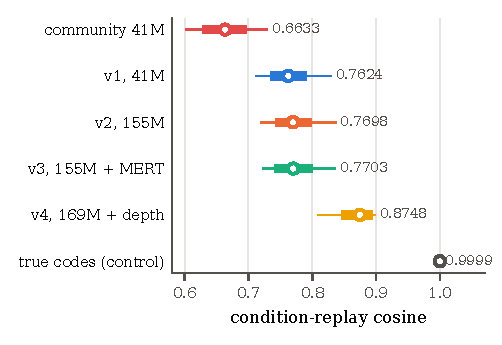
\includegraphics[width=\columnwidth]{figures/replay.pdf}
  \caption{Condition-replay cosine over the 130 held-out tracks: mean (marker), 5th to 95th percentile (bar), min to max (line). The v4 (depth-causal) distribution is separated from every independent-head model.}
  \label{fig:replay}
\end{figure}

\subsection{Token agreement}

Table~\ref{tab:matched} scores the four models on exact agreement with the sampled codes at the matched step 17,500, the last checkpoint common to all runs. The loss column is the training objective at KL weight 0.25. The four accuracy columns give top-1 and top-5 inclusion of the sampled code, first for the semantic codebook and then pooled over the seven acoustic codebooks. Semantic top-1 rises from 41.0\% to 43.2\% and semantic top-5 from 78.4\% to 80.5\% across the family, while pooled acoustic top-1 stays between 7.2\% and 7.7\% for every model; the acoustic columns are the ones that do not follow the replay metric of Tab.~\ref{tab:replay}, which is the observation Sec.~\ref{sec:analysis} builds on.

\begin{table}[tb]
\centering
\small
\caption{Exact-token metrics at the matched step 17,500 (percent).}
\label{tab:matched}
\adjustbox{max width=\columnwidth}{
\begin{tabular}{lrrrrr}
\toprule
Model & Loss & Sem. top-1 & Sem. top-5 & Ac. top-1 & Ac. top-5 \\
\midrule
v1, 41M & 5.3379 & 41.03 & 78.38 & 7.17 & 20.94 \\
v2, 155M & 5.2646 & 42.86 & 80.17 & 7.62 & 21.98 \\
v3, 155M + MERT & 5.2602 & 43.03 & 80.48 & 7.65 & 22.02 \\
v4, 169M + depth & 3.9882 & 43.16 & 80.51 & 7.30 & 19.88 \\
\bottomrule
\end{tabular}
}
\end{table}


The v4 loss is lower than the other three rows because the acoustic terms of v4 are conditioned on the true earlier codes during scoring, so they are not comparable with the independent-head rows and should not be read as a better fit. Re-evaluating the released weights on the same held-out split reproduces every published row within 0.003 in loss and 0.001 in accuracy (Sec.~\ref{app:extra}).

\subsection{Compression characteristics}

The code stream carries $14 + 7 \times 10 = 84$ bits per frame at 25 Hz, 2.1 kbit/s, against 128 latent channels at 86.13 Hz on the DAV side and 1,411 kbit/s for the 16-bit stereo waveform. The encoder is therefore a lossy map by construction, and the tolerance of the downstream conditioning to alternative tuples (Sec.~\ref{sec:analysis}) is what lets a 2.1 kbit/s stream condition the generator at 0.87 cosine. Encoding runs at 64$\times$ real time on one RTX 3090, 5.6 s for six minutes of stereo audio, four fifths of it in the frozen DAV encoder.

\subsection{Ablation studies}

Each model in Tab.~\ref{tab:family} differs from the one before it by one named change, so the rows of Tab.~\ref{tab:replay} read as an ablation, and because every model is scored on the same 130 tracks the differences are paired. Table~\ref{tab:bootstrap} gives each difference of interest with a percentile bootstrap interval: the first column names the pair, the second is the mean of the per-track differences, the third is the 95\% interval from 10,000 resamples of the 130 tracks, and the last column counts the tracks on which the first model beats the second. Three of the five comparisons improve every one of the 130 tracks: v1 over the community encoder (+0.099), v2 over v1 (+0.007) and v4 over either v2 or v3 (+0.105 and +0.1045). The MERT comparison is the exception, +0.0004 with an interval that touches zero and only 77 of 130 tracks improved, which is why we describe it as negligible for a single run rather than as an improvement.

\begin{table}[tb]
\centering
\small
\caption{Paired differences in condition-replay cosine over the same 130 tracks, with percentile bootstrap intervals (10,000 resamples).}
\label{tab:bootstrap}
\adjustbox{max width=\columnwidth}{
\begin{tabular}{lrrr}
\toprule
Comparison & Mean difference & 95\% interval & Tracks improved \\
\midrule
v1 minus community 41M & +0.0991 & [+0.0968, +0.1014] & 130 of 130 \\
v2 minus v1 & +0.0074 & [+0.0070, +0.0078] & 130 of 130 \\
v3 minus v2 & +0.0004 & [+0.0000, +0.0008] & 77 of 130 \\
v4 minus v2 & +0.1050 & [+0.1014, +0.1086] & 130 of 130 \\
v4 minus v3 & +0.1045 & [+0.1009, +0.1082] & 130 of 130 \\
\bottomrule
\end{tabular}
}
\end{table}


Two caveats limit what the ablation isolates. The larger v2 configuration improves every token metric over v1 by one to two points and replay cosine by 0.007, but v1 also used a different learning-rate schedule (a reheating cosine against linear warm-up and decay) and a different head count, so this comparison does not isolate width, and we read it only as evidence that capacity was not the main limit. MERT alignment (v2 to v3) changes token metrics by 0.03 to 0.3 points and replay by 0.0004, too little to justify a training dependency, and v4 therefore builds on the v2 encoder rather than on v3. The causal depth decoder (v4 against v2, the structurally matched comparison) improves semantic agreement marginally, \emph{lowers} free-running acoustic top-1 by 0.32 points, and raises replay cosine by 0.105, the only change that moves the downstream metric substantially. v4 also carries 22.1M more parameters than v2 in the decoder; a parameter-matched independent-head model or a non-causal decoder of the same size, which would separate conditioning from capacity, was not trained (Sec.~\ref{sec:limitations}).

Two implementation choices were also ablated by measurement. Fused attention is 3.6$\times$ faster forward and 2.8$\times$ faster backward at the temporal stack's shape (batch 16, 17 heads, length 128) and 2.9$\times$ and 3.8$\times$ slower at the depth decoder's shape (batch 2,048, 8 heads, length 8), so the two stacks use different kernels. The segment form of the pooling operator is 11$\times$ to 18$\times$ cheaper to assemble per batch than the dense matrix and equal on device (Sec.~\ref{app:extra}).
